\documentclass{report}

% Packages nécessaires
\usepackage[utf8]{inputenc}
\usepackage[T1]{fontenc}
\usepackage[french]{babel}
\usepackage{titlesec}
\usepackage{tocloft}
\usepackage{lipsum} % Package de remplissage de texte (à retirer dans le rapport final)
\usepackage{graphicx}
\usepackage{float} % pour l'option de placement [H]
\usepackage[colorlinks=true, linkcolor=blue, citecolor=green]{hyperref}
\usepackage{lipsum}
\usepackage{wrapfig}   % Pour l'enroulement du texte autour des images
\usepackage{array}
\usepackage{tikz}
\usepackage{listings}
\usepackage{xcolor}
\usepackage{graphicx}
\usepackage{pdfpages}
\usepackage{background}
\usepackage{amsmath}
\usepackage{verbatim} %permet de commenter des codes entiers
\usepackage{listings}
\usepackage[utf8]{inputenc}
\usepackage{listings}
\usepackage[T1]{fontenc} % Aide à la gestion des caractères européens

\lstset{
  language=Python,
  inputencoding=utf8,       % On essaie l'utf8
  extendedchars=true,
  % Cette ligne ci-dessous est MAGIQUE : elle remplace les caractères problématiques 
  % par leur version LaTeX sans faire planter le moteur
  literate={é}{{\'e}}1 {è}{{\`e}}1 {à}{{\`a}}1 {ç}{{\c{c}}}1 {œ}{{\oe}}1 {ù}{{\`u}}1 {É}{{\'E}}1 {È}{{\`E}}1 {À}{{\`A}}1 {°}{{$^\circ$}}1,
  breaklines=true,
  breakatwhitespace=true,
  basicstyle=\small\ttfamily,
  columns=fullflexible,
  keepspaces=true
}

%Permet de définir les codes en couleur
\definecolor{codegreen}{rgb}{0,0.6,0}
\definecolor{codegray}{rgb}{0.5,0.5,0.5}
\definecolor{codepurple}{rgb}{0.58,0,0.82}
\definecolor{backcolour}{rgb}{0.95,0.95,0.92}

%Pour que les codes soient en couleur
\lstdefinestyle{pythonstyle}{
    backgroundcolor=\color{backcolour},
    commentstyle=\color{codegreen},
    keywordstyle=\color{blue},
    numberstyle=\tiny\color{codegray},
    stringstyle=\color{codepurple},
    basicstyle=\ttfamily\footnotesize,
    breaklines=true,
    captionpos=b,
    keepspaces=true,
    numbers=left,
    numbersep=5pt,
    showspaces=false,
    showstringspaces=false,
    showtabs=false,
    tabsize=2,
    language=Python
}
%Indique que la coloration des codes doit suivre celle d'un code Python
\lstset{style=pythonstyle}

% Configuration de la page
\usepackage[a4paper, left=2.5cm, right=2.5cm, top=2.5cm, bottom=2.5cm]{geometry}

% Configuration des titres des sections et sous-sections
\titleformat{\chapter}[display]
  {\normalfont\huge\bfseries}{\chaptertitlename\ \thechapter}{20pt}{\Huge}
\titleformat{\section}
  {\normalfont\Large\bfseries}{\thesection}{1em}{}
\titleformat{\subsection}
  {\normalfont\large\bfseries}{\thesubsection}{1em}{}

% Configuration de la table des matières
\renewcommand{\cftchapfont}{\bfseries}
\renewcommand{\cftsecfont}{\normalfont}
\renewcommand{\cftsubsecfont}{\normalfont}
\renewcommand{\cftchappagefont}{\bfseries}
\renewcommand{\cftsecpagefont}{\normalfont}
\renewcommand{\cftsubsecpagefont}{\normalfont}
\setlength{\cftbeforetoctitleskip}{0pt}
\setlength{\cftaftertoctitleskip}{10pt}
\renewcommand{\contentsname}{Table des matières}

\begin{document}

% Désactiver le fond
\backgroundsetup{contents={}}

% Insérer le PDF

\includepdf[pages=-, fitpaper=true]{Template.pdf}

% Réactiver le fond
% Pour avoir le petit dessin de l'INSA en bas à droite de chaque page
\backgroundsetup{
scale=1,
angle=0,
opacity=1,
color=black,
contents={\begin{tikzpicture}[remember picture,overlay]
\node at ([xshift=-0.8in,yshift=0.8in] current page.south east)
{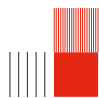
\includegraphics[scale=0.8]{images/pattern.png}};
\end{tikzpicture}}
}

\begin{comment}
% --- PAGE DE TITRE ---
\begin{titlepage}
    \centering
    \noindent 
    \begin{minipage}{0.45\textwidth}
        
\includegraphics[width=0.8\linewidth]{images/logo_INSA.png} 
    \end{minipage}%
    \hfill 
    \begin{minipage}{0.45\textwidth}
        \flushright 
        
\includegraphics[width=0.8\linewidth]{images/tescan_logo.png} 
    \end{minipage}

    \vspace*{2cm} 
    {\Huge\bfseries Rapport de Projet Multidisciplinaire \par}
    \vspace{1cm}
    {\huge Modélisation du Quadrupôle d'Okayama par BEM \par}
    \vspace{0.4cm}
    {\large (\textit{Boundary Element Method}) \par}
    \vspace{2cm}

    {\Large \textbf{Zoé \textsc{Nonon} --- Louise \textsc{Lammertyn}} \par}
    \vspace{0.2cm}
    {\large $4^{\text{ème}}$ année Génie Physique \par}
    
    \vspace{2.5cm}

    {\large \textbf{Tuteurs :}} \par
    \vspace{0.5cm}
    {\large
    \begin{tabular}{l}
        Florent \textsc{Houdellier} \\
        Lucile \textsc{Berdoux Durieux} \\
        Jean-Baptiste \textsc{Mellier} \\
        Pier-Francesco \textsc{Fazzini}
    \end{tabular}
    } \par
    
    \vfill 
    {\large Année universitaire 2025-2026 \par}
    \vspace{0.8cm}
    {\Large \textbf{Institut National des Sciences Appliquées de Toulouse} \par}
    \vspace{0.5cm}
    {\large \today \par}
\end{titlepage}
\end{comment}

%Pour les remerciements
\begin{center}
    \thispagestyle{empty} % Pas de numéro de page sur cette page
    \vspace*{\fill}
    \section*{Remerciements}
    \addcontentsline{toc}{chapter}{Remerciements}
    
    Ce projet multidisciplinaire n'aurait pu voir le jour sans l'aide de...
    
    \vspace*{\fill}
\end{center}
\clearpage

% Résumé concis, souvent utilisé pour donner un aperçu rapide du contenu d'une recherche ou d'un article académique.
\begin{center}
    \thispagestyle{empty} % Pas de numéro de page sur cette page
    \vspace*{\fill}
    \section*{Abstract}
    \addcontentsline{toc}{chapter}{Remerciements}
    
    Ce document est le rapport final du projet multidisciplinaire de 4ème année en Génie Physique de l'INSA Toulouse. Il a pour but d'expliquer en détail la démarche que nous avons suivit 
    afin de mener à bien ce projet. Ce document retrace donc le contexte, l'organisation mais aussi toutes les équations que nous avons dû étudier. 
    
    \vspace*{\fill}
\end{center}
\clearpage

% Table des matières
\tableofcontents

\chapter{Introduction}


\section{Contexte}
Dans le cadre du projet multidisciplinaire de 4ème du Génie physique de l'INSA Toulouse, nous devons modéliser les lentilles électrostatiques quadrupolaires 
d'un FIB (Focused Ion Beam) en utilisant une méthode mathématique appelée la méthode des éléments de frontière. Pour ce faire, nous devons écrire un code Python 
en utilisant notamment la bibliothèque BEMPP. Afin de pouvoir réaliser cette entreprise, il est nécessaire de comprendre l'optique des particules chargées dans le contexte
de lentilles quadrupolaires. 

\section{Présentation du projet}
L’optique des particules chargées est une science qui sert à comprendre et à maîtriser la 
trajectoire de faisceaux électroniques ou ioniques. Cette discipline a permis de créer de 
nombreux instruments comme notamment les SEM (Scanning electron microscop = 
microscope électronique à balayage) et les FIB (focused ion beam = faisceau d’ions focalisé) 
utilisés dans de nombreuses disciplines comme la médecine ou la microélectronique.  
Plus spécifiquement, un FIB est composé de plusieurs éléments dont notamment des 
lentilles. En effet, celles-ci permettent de guider la trajectoire du faisceau ionique au sein de 
l’instrument et de corriger les différentes aberrations de celui-ci. Il est donc primordial de 
comprendre et maîtriser ces objets afin de rendre le FIB le plus performant possible.  

\begin{figure}[H]
\centering
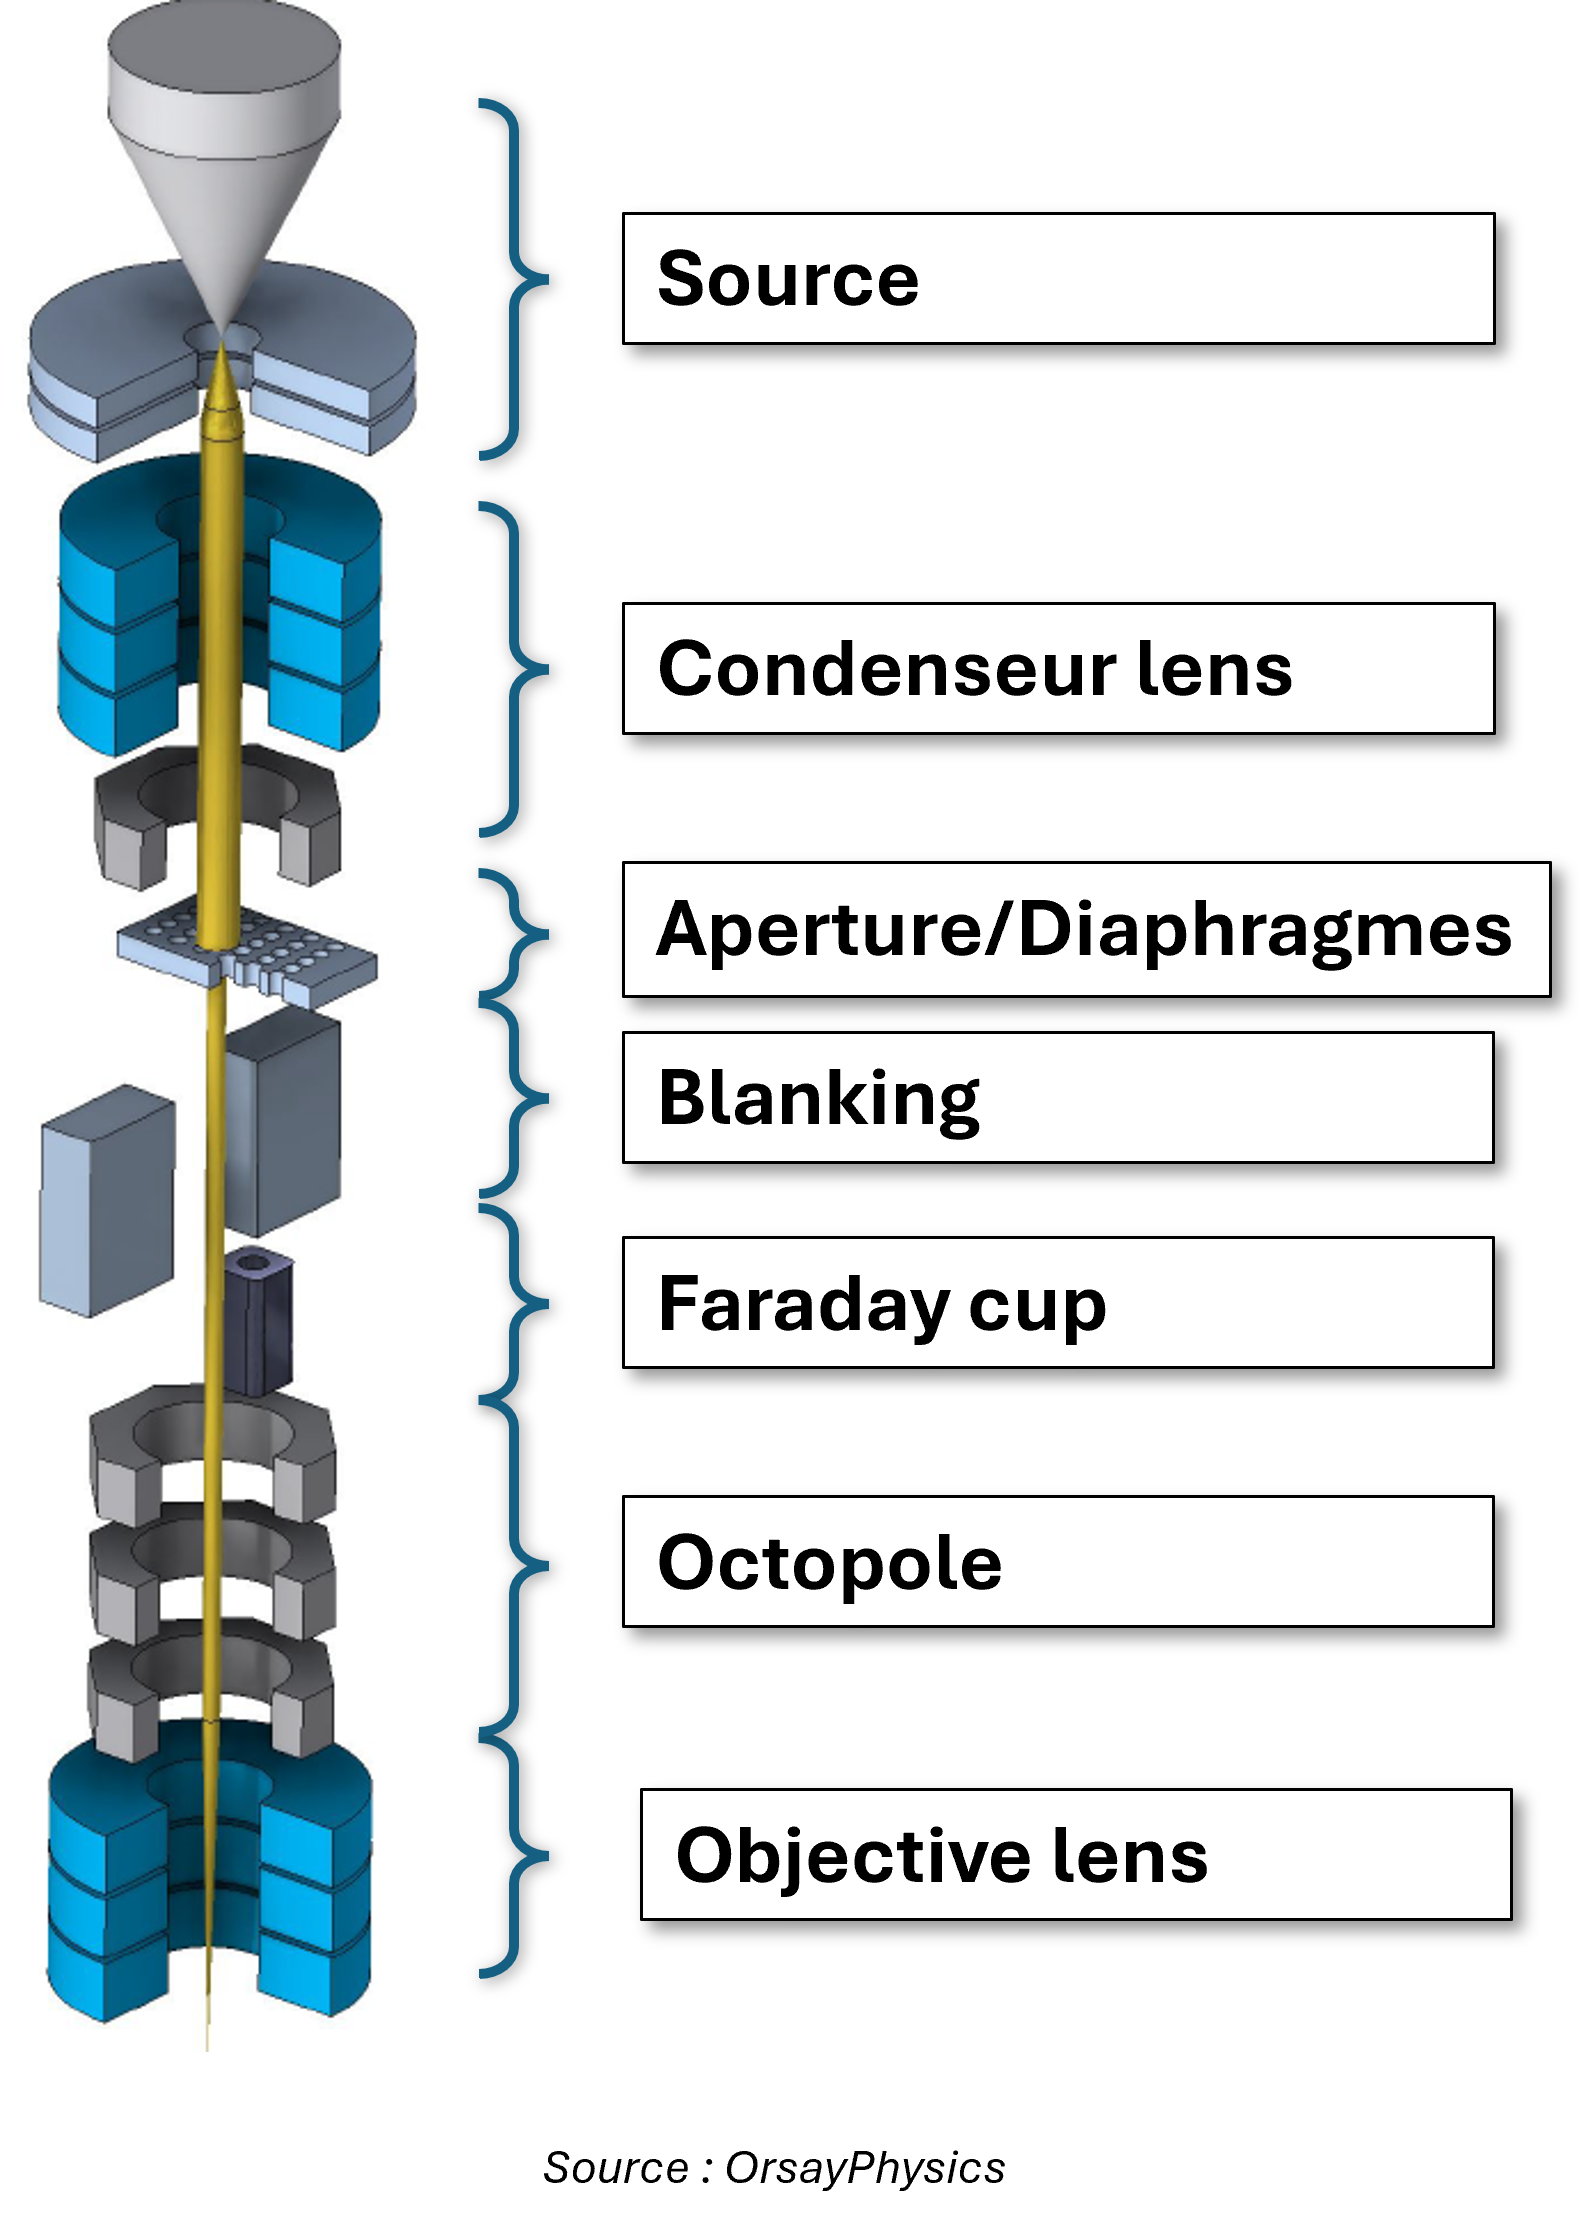
\includegraphics[width=0.3\linewidth]{images/Schema_Colonne_FIB_OP.png} 
\caption{Schéma d’un FIB}
\label{fig:fib}
\end{figure}


Cependant, la fabrication de ces instruments peut parfois être longue et coûteuse. Pour 
pallier ce problème, l’utilisation de modèles s’avère utile. C’est dans ce cadre que notre 
projet multidisciplinaire s’inscrit et est intitulé: “Modélisation de lentilles multipolaires 
électrostatiques par Boundary Element Method”.  
Comme évoqué précédemment, les lentilles permettent de guider la trajectoire du faisceau 
ionique. Il existe plusieurs types de lentilles: les lentilles électrostatiques et les lentilles 
magnétiques. Dans le cas que nous étudions, le FIB est composé de lentilles 
électrostatiques.  
Ces lentilles électrostatiques peuvent présenter différentes configurations. On parle en effet 
de lentilles rondes/monopolaires (un seul potentiel), de lentilles dipolaires (deux potentiels), 
de lentilles quadrupolaires (quatres potentiels), etc. Notre étude portera plus particulièrement 
sur les lentilles quadrupolaires.  


\begin{figure}[H]
\centering
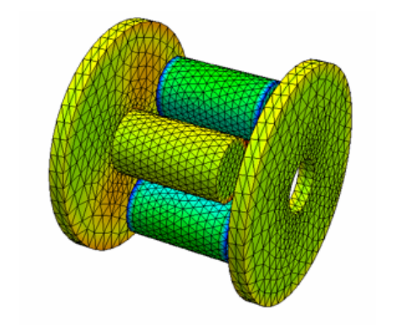
\includegraphics[width=0.4\linewidth]{images/Quadrupole_CEOS.png} 
\caption{Modélisation d’une lentille quadrupolaire électrostatique}
\label{fig:quad}
\end{figure}

Le principe de ce projet multidisciplinaire est de créer un code OpenSource permettant de 
modéliser des lentilles quadrupolaires électrostatiques.  
Cette étude s’inscrit dans la continuité de deux projets multidisciplinaires précédents. Le 
premier projet consistait à prendre en main un code déjà existant permettant de modéliser un 
cas simple de lentilles électrostatiques (les lentilles de Einzel). Le second avait pour but de 
créer un algorithme permettant d’optimiser ces lentilles.  
Notre objectif est donc de continuer ce projet en l’adaptant aux lentilles quadrupolaires.  
Ce code OpenSource a pour vocation de devenir une ressource utilisable dans le monde de 
l’optique des particules chargées. Ce projet permettrait notamment à l’entreprise avec 
laquelle nous travaillons, Tescan, de disposer d’un code facilitant la modélisation de lentilles 
multipolaires électrostatiques.  

\section{Objectifs du projet}
\subsection{Objectif 1 - Prise en main de BEMPP}
Le premier objectif de ce projet est de se familiariser avec BEMPP, “Boundary element 
method Python package”, une bibliothèque open-source de calcul par éléments de frontière. 
Celle-ci permet de résoudre des problèmes électrostatiques, acoustiques et 
électromagnétiques à l’aide d’une formulation intégrale. 
Dans notre cas, BEMPP nous permettra de mailler les électrodes des lentilles 
électrostatiques et de calculer le potentiel en chaque point du volume. 
Dans un premier temps, nous appliquerons BEMPP dans des cas simples tels que des 
lentilles rondes. Nous connaissons en effet les résultats attendus car cela a déjà fait l’objet 
d’un projet multidisciplinaire.  

\subsection{Objectif 2 - Algorithme de la décomposition multipolaire}
Le deuxième objectif est de comprendre la méthode de calcul mathématiques qui va nous 
permettre de décomposer le potentiel donné par BEMPP.  
Cette étude est essentielle pour retrouver le potentiel électrostatique en n’importe quel point 
du volume du système. En effet, la décomposition du potentiel est primordiale pour résoudre 
les équations de la trajectoire, donc connaître le potentiel électrostatique en n’importe quel 
point du volume, et connaître les aberrations d’un tel système.  

\subsection{Objectif 3 - EXtraction du potentiel}
Une fois les outils précédents maîtrisés, nous pourrons les appliquer au cas spécifique des 
lentilles quadrupolaires électrostatiques. Il sera alors nécessaire de mailler les électrodes du 
quadrupole et d’appliquer le code Python développé afin d’obtenir le potentiel électrostatique 
à l’intérieur du système optique. 
Pour vérifier la justesse de nos calculs, nous pourrons comparer nos résultats à ceux du 
quadrupole d’Okayama qui a été développé par une équipe de l’université d’Okayama au 
Japon.  

\subsection{Objectif 4 - Décomposition des différentes contributions}
Une fois le potentiel total obtenu, il sera possible d’analyser les trajectoires des particules. 
Pour cela, nous nous aiderons de l'algorithme de calcul évoqué dans l’objectif 2. Cette 
approche permettra d’effectuer la décomposition du potentiel $\Phi$, d’en déduire celle de l’indice 
optique µ, et ainsi d’accéder aux aberrations optiques du système et à la résolution des 
équations du mouvement.  
Les équations du mouvement seront résolues à l’aide de méthodes d’intégration numérique 
de type Runge–Kutta d’ordre 4. 

\section{Livrables}
Le premier livrable sera un algorithme de décomposition du potentiel. 
Le livrable suivant sera un code fonctionnel de modélisation de lentilles quadrupolaires 
électrostatiques, accompagné d’un manuel d’explication, détaillant le fonctionnement de 
chaque fonction, des classes et leur utilisation. 
Dans un dernier temps, nous fournirons une comparaison des résultats de notre code avec 
ceux du quadrupôle d’Okayama, dont nous connaissons déjà les résultats. 
De plus, notre code étant open-source, nous fournirons un dépôt GitHub regroupant le code 
et toute la documentation associée pour qu’il puisse être utilisé. 


\chapter{Démarche générale}
\section{Principe de moindre action}
Le commencement de ce raisonnement est le principe de moindre action qui s'exprime comme 
\[
\delta S = \int_{S0}^{S1} \vec{p}\,\frac{\vec{r}}{dS} \, \mathrm{d}s = 0
\]
\\
On peut alors montrer que 
\[
\delta S = \int_{S0}^{S1} \mu\,\mathrm{d}z = 0
\]
\\
Comme le quadrupole que nous utilisons est composé UNIQUEMENT de lentilles électrostatiques, on peut écrire
\[
\mu = \sqrt{\phi \, (1+x'^2+y'2)}
\]
avec $\mu$ l'indice optique, $\phi$ le potentiel électrostatique et x' et y' les dérivées de x et y par
rapport à z.

\section{Equations d'Euler-Lagrange}
Les équations d'Euler-Lagrange sont des équations équivalentes au principe de moindre action, sous forme 
différentielle. On peut ainsi noter 
\[
\frac{\partial \mu }{\partial x}-\frac{d}{dz}\left(\frac{\partial \mu }{\partial x'}\right)=0
\]
\[
\frac{\partial \mu }{\partial y}-\frac{d}{dz}\left(\frac{\partial \mu }{\partial y'}\right)=0
\]

\section{Décomposition du potentiel}
Une fois les équations d'Euler-Lagrange exprimées, il est utile de décomposer le potentiel $\phi$ afin de 
séparer les solutions de ces équations en fonction de leur dépendance aux différents ordres de x et y. 
\\
\\
On peut ainsi décomposer ce potentiel en série de Fourrier et en série de Taylor. 
\\
\\
Dans le cadre de notre étude, c'est-à-dire dans le cadre d'un quadrupole, on observe une 2$\pi$ périodicité 
du potentiel selon $\theta$.
On peut donc décomposer le potentiel comme une série de Fourrier. Celle-ci, de part sa périodicité, représente 
donc les symétries du système. On obtient alors 

\[
\phi ({\color{red}r},{\color{blue}\theta},{\color{green}z})=\sum\limits_{\nu =0}^{\infty} \phi_\nu ({\color{red}r},{\color{blue}\theta},{\color{green}z})
\]

avec 

\[
\phi_\nu ({\color{red}r},{\color{blue}\theta},{\color{green}z})=a_\nu cos(\nu{\color{blue}\theta})+b_\nu sin(\nu {\color{blue}\theta})
\]
\\ 
Ainsi, le potentiel $\phi ({\color{red}r},{\color{blue}\theta},{\color{green}z})$ est composé d'une somme de fonctions dépendantes de 
${\color{red}r}$, ${\color{blue}\theta}$ et ${\color{green}z}$. On remarque alors que les variables 
({\color{red}r}, {\color{green}z}) et ${\color{blue}\theta}$ sont séparées sous la forme suivante: 
\[
\phi_\nu ({\color{red}r},{\color{blue}\theta},{\color{green}z})=f({\color{red}r},{\color{green}z})\times g({\color{blue}\theta})
\]
Il est nécessaire que le potentiel électrostatique satisfasse l'équation de Laplace $\Delta \phi(\vec{r})=0$. On peut
exprimer cette même équation en coordonnées cylindriques comme  
\[
\frac{1}{r} \frac{\partial}{\partial r} \left(r \frac{\partial \phi}{\partial r} \right) + \frac{1}{r^2} \frac{\partial^{2}}{\partial \theta ^2}
+ \frac{1}{r^2} \frac{\partial^{2}}{\partial z ^2}=0
\]
En injectant $\phi ({\color{red}r},{\color{blue}\theta},{\color{green}z})=\sum\limits_{\nu =0}^{\infty} \phi_\nu ({\color{red}r},{\color{blue}\theta},{\color{green}z})$
dans l'équation précédente, on obtient l'équation suivante

\[
\sum\limits_{\nu =0}^{\infty} \left(cos(\nu {\color{blue}\theta}) \left(\frac{\partial^{2} a_\nu}{\partial {\color{red}r}^2} + \frac{1}{{\color{red}r}} 
\frac{\partial a_\nu}{\partial {\color{red}r}} + \frac{\partial^{2} a_\nu}{\partial {\color{green}z}^2} - a_\nu \frac{\nu ^2}{{\color{red}r}^2}\right) 
+ sin(\nu {\color{blue}\theta}) \left(\frac{\partial^{2} b_\nu}{\partial {\color{red}r}^2} + \frac{1}{{\color{red}r}} \frac{\partial b_\nu}{\partial {\color{red}r}} 
+ \frac{\partial^{2} b_\nu}{\partial {\color{green}z}^2}- b_\nu \frac{\nu ^2}{{\color{red}r}^2}\right)\right) = 0
\]

\
\\
On peut alors montrer que cette équation peut être résolue $\forall {\color{red}r}$, si on vérifie
\[
\frac{\partial^{2} a_\nu}{\partial {\color{red}r}^2} + \frac{1}{{\color{red}r}} 
\frac{\partial a_\nu}{\partial {\color{red}r}} + \frac{\partial^{2} a_\nu}{\partial {\color{green}z}^2} - a_\nu \frac{\nu ^2}{{\color{red}r}^2}=0
\]

et 
\[
\frac{\partial^{2} b_\nu}{\partial {\color{red}r}^2} + \frac{1}{{\color{red}r}} \frac{\partial b_\nu}{\partial {\color{red}r}} 
+ \frac{\partial^{2} b_\nu}{\partial {\color{green}z}^2}- b_\nu \frac{\nu ^2}{{\color{red}r}^2}=0 
\]

\
\\
Il est maintenant utile de développer les fonctions $a_\nu ({\color{red}r},{\color{green}z})$ et $b_\nu ({\color{red}r},{\color{green}z})$
en série de Taylor, dans le but de séparer la dépendance des variables ${\color{red}r}$ et ${\color{green}z}$. 
Dans le cadre de notre étude, on considère des conditions paraxiales, c'est-à-dire des conditions où les rayons sont proches de l'axe optique. On effectue
donc le développement en série de Taylor pour ${\color{red}r}=0$.
\
\\
{\textit{
{\underline{Rappel:}} 
Une série de Taylor $f(x)$ en $x=b$ s'exprime comme $f(x)=\sum\limits_{n=0}^{\infty} a_n(x-b)^n$. 
}}
\
\\
On peut ainsi écrire 
\[
A_\nu ({\color{red}r},{\color{green}z})=\sum\limits_{i=0}^{\infty} a_{i\nu} ({\color{green}z}) \times ({\color{red}r})^{\nu + i}
\]
et 
\[
B_\nu ({\color{red}r},{\color{green}z})=\sum\limits_{i=0}^{\infty} b_{i\nu} ({\color{green}z}) \times ({\color{red}r})^{\nu + i}
\]
\
\\ 
On pose alors $A_{\nu 0} ({\color{green}z})=\Phi_{\nu {\color{red}r}}$ et $B_{\nu 0} ({\color{green}z})=\Phi_{\nu i}$, les composantes 
de Fourrier du potentiel sur l'axe. On peut alors insérer les coefficients de la série de Taylor dans les composantes de la série de 
Fourrier. On obtient alors 
\[
A_\nu ({\color{red}r},{\color{green}z})=\sum\limits_{\lambda=0}^{\infty} \frac{(-1)^{\lambda}\times (\nu !)}{4^{\lambda}\times \lambda !\times (\lambda +\nu)!}
\times {\color{red}r}^{\nu +2\lambda} \times \Phi_{\nu {\color{red}r}}^{[2\lambda]}({\color{green}z}) 
\]
et 
\[
B_\nu ({\color{red}r},{\color{green}z})=\sum\limits_{\lambda=0}^{\infty} \frac{(-1)^{\lambda}\times (\nu !)}{4^{\lambda}\times \lambda !\times (\lambda +\nu)!}
\times {\color{red}r}^{\nu +2\lambda} \times \Phi_{\nu i}^{[2\lambda]}({\color{green}z}) 
\]
% dans les deux expression précédentes, quelles sont les bornes des sommes: i ou lambda? 
\
\\
On peut alors écrire le potentiel $\phi ({\color{red}r},{\color{blue}\theta},{\color{green}z})$ comme une somme polynomiale avec les dérivées du potentiel pris sur 
l'axe optique comme coefficients des polynômes. On a alors 

\[
\phi ({\color{red}r},{\color{blue}\theta},{\color{green}z})= \sum\limits_{\nu =0}^{\infty}
\sum\limits_{\lambda=0}^{\infty} \frac{(-1)^{\lambda}\times (\nu !)}{4^{\lambda}\times \lambda !\times (\lambda +\nu)!}
\times {\color{red}r}^{\nu +2\lambda} \times \left(\Phi_{\nu {\color{red}r}}^{[2\lambda]}({\color{green}z})\times cos(\nu{\color{blue}\theta}) + 
\Phi_{\nu i}^{[2\lambda]}({\color{green}z})\times sin(\nu{\color{blue}\theta}) \right)
\]
\section{Décomposition des différentes contributions}
Une fois le potentiel  $\phi ({\color{red}r},{\color{blue}\theta},{\color{green}z})$ décomposé, on peut l'injecter dans l'équation 
\[
\mu = \sqrt{\phi \, (1+x'^2+y'2)}=\sqrt{\phi} \, \sqrt{1+x'^2+y'2}
\]
afin de déterminer les différentes contributions qui composent l'indice optique. 
\
\\
Cependant, on remarque que l'indice optique $\nu$ dépend à l'ordre 2 des dérivées de x et y. 
Dans la démarche de décomposer les différentes contributions de l'indice optique, il est nécessaire d'effectuer un développement limité de 
\[
\sqrt{1+x'^2+y'2}
\] 
\
On pose X=$x'^2$ +$y'^2$ afin d'effectuer un changement de variable. 
\
\\
\\
{\textit{
{\underline{Rappel:}} 
Le développement limité d'une racine carrée est $\sqrt{1+X}=1+\frac{x}{2}-\frac{x^2}{8}+...$. 
}}
\
\\
\\
On obtient ainsi les différentes contributions de l'indice optique $\mu=\mu_0+\mu_1+\mu_2+\mu_3+\mu_4+\mu_5+...$. 
\
\\
Les composantes $\mu_0$, $\mu_1$ et $\mu_2$ composent la partie paraxiale de l'équation tandis que les 
termes d'ordres supérieurs correspondent aux aberrations. $\mu_0$ correspond à l'axe optique du système. 
$\mu_2$ correspond au paraxial du système optique.  
\
\\
On note que la paraxialité a une dépendance à l'ordre 2 des variable x et y car en optique, le front d'onde est sphérique. Le front d'onde est une surface 
d'égale phase d'une onde, c'est-à-dire que les points qui composent cette sphère ont mis le même temps de parcours depuis la source. Ainsi, dans des conditions parfaites, où les aberrations 
de front d'onde n'existent pas, le front d'onde est parfaitement sphérique, ce qui explique la dépendance d'ordre 2 des variables x et y. 
\\
Lorsque le front d'onde n'est plus parfaitement sphérique, autrement dit quand le système connait une perturbation, tous les points du front d'onde ne vont plus focaliser au même endroit. 
On obtient ainsi des aberrations. Ces dernières correspondent à tous les termes d'ordres supérieurs à 2 de la somme infini de $\nu$. b
\
\section{Reconstruction de la décomposition du potentiel}
\subsection{Extraction du potentiel}
A l'aide de la bibliothèque Python BEMPP $(Boundary Element Method Python Package)$, on peut extraire le potentiel $\phi ({\color{red}r},{\color{blue}\theta},{\color{green}z})$ 
en tout point de l'espace. Comme vu dans la partie précédente, il est important de décomposer le potentiel afin de pouvoir séparer la contribution des différents ordres. Une fois le potentiel extrait,
il faut donc trouver les différentes composantes de la décomposition du potentiel.

\subsection{Composantes multipolaires}
\subsubsection{Equations}
On peut retouver les composantes multipolaires à l'aide de la formule 
\[
\Phi_{\nu}= \frac{2-\delta_{0\nu}}{\nu!}\left.
(\frac{\partial^{\nu} \phi}{\partial \bar w^{\nu}})
\right|_{ w=0}.
\]
où $\nu$ est l'ordre du terme multipolaire et $\delta_{0\nu}$ le symbole de Kronecker.
\\
Pour un développement limité à l'ordre $N$ en ${\color{red}r}$, les valeurs admissibles de $\lambda$ sont déterminées par la condition
\[
2\lambda + \nu \le N
\]
Dans le cadre de ce travail, on se limite à $N=4$ et $\nu \le 2$, ce qui conduit aux valeurs suivantes : $\lambda = 0,1,2$ pour $\nu=0$ et $\lambda = 0,1$ pour $\nu=1,2$.
\\
\\
On peut alors calculer les différents ordres des composantes multipolaires: 
\paragraph{Cas \(\nu = 0\) (monopôle)}
\
\\
On a \(\delta_{00} = 1\), d'où
\[
\Phi_0(z) = \frac{2 - \delta_{00}}{0!} \left. \frac{\partial^{0} \phi}{\partial \bar{w}^{0}} \right|_{w=0} = \phi(x, y, z)\big|_{w=0}.
\]

\paragraph{Cas \(\nu = 1\) (dipôle)}
\
\\
On a \(\delta_{01} = 0\), d'où
\[
\Phi_1(z) = \frac{2 - \delta_{01}}{1!} \left. \left( \frac{\partial \phi}{\partial \bar{w}} \right) \right|_{w=0} = 2 \left. \frac{\partial \phi}{\partial \bar{w}} \right|_{w=0}.
\]

\paragraph{Cas \(\nu = 2\) (quadrupôle)}
\
\\
On a \(\delta_{02} = 0\), d'où
\[
\Phi_2(z) = \frac{2 - \delta_{02}}{2!} \left. \frac{\partial^{2} \phi}{\partial \bar{w}^{2}} \right|_{w=0} = \frac{1}{2} \left. \frac{\partial^{2} \phi}{\partial \bar{w}^{2}} \right|_{w=0}.
\]

\paragraph{Cas \(\nu = 3\) (hexapôle)}
\
\\
On a \(\delta_{03} = 0\), d'où
\[
\Phi_3(z) = \frac{2 - \delta_{03}}{3!} \left. \frac{\partial^{3} \phi}{\partial \bar{w}^{3}} \right|_{w=0} = \frac{1}{3} \left. \frac{\partial^{3} \phi}{\partial \bar{w}^{3}} \right|_{w=0}.
\]

\paragraph{Cas \(\nu = 4\) (octopôle)}
\
\\
On a \(\delta_{04} = 0\), d'où
\[
\Phi_4(z) = \frac{2 - \delta_{04}}{4!} \left. \frac{\partial^{4} \phi}{\partial \bar{w}^{4}} \right|_{w=0} = \frac{1}{12} \left. \frac{\partial^{4} \phi}{\partial \bar{w}^{4}} \right|_{w=0}.
\]

\paragraph{Cas général}
\
\\
On obtient finalement avec \(\bar{w} = x - iy\) et \(\frac{\partial}{\partial \bar{w}} = \frac{1}{2}\left(\frac{\partial}{\partial x} + i\frac{\partial}{\partial y}\right)\) que

\[
\begin{aligned}
\Phi_0(z) &= \phi(x, y, z)\big|_{x=y=0}, \\[0.4em]
\Phi_1(z) &= \left. \left( \frac{\partial \phi}{\partial x} + i \frac{\partial \phi}{\partial y} \right) \right|_{x=y=0}, \\[0.6em]
\Phi_2(z) &= \left. \frac{1}{8} \left( \frac{\partial^{2} \phi}{\partial x^{2}} - \frac{\partial^{2} \phi}{\partial y^{2}} - 2i \frac{\partial^{2} \phi}{\partial x \partial y} \right) \right|_{x=y=0}, \\[0.6em]
\Phi_3(z) &= \left. \frac{1}{24} \left( \frac{\partial^{3} \phi}{\partial x^{3}} - 3 \frac{\partial^{3} \phi}{\partial x \partial y^{2}} - 3i \frac{\partial^{3} \phi}{\partial x^{2} \partial y} + i \frac{\partial^{3} \phi}{\partial y^{3}} \right) \right|_{x=y=0}, \\[0.6em]
\Phi_4(z) &= \left. \frac{1}{192} \left( \frac{\partial^{4} \phi}{\partial x^{4}} - 6 \frac{\partial^{4} \phi}{\partial x^{2} \partial y^{2}} + \frac{\partial^{4} \phi}{\partial y^{4}} - 4i \frac{\partial^{4} \phi}{\partial x^{3} \partial y} + 4i \frac{\partial^{4} \phi}{\partial x \partial y^{3}} \right) \right|_{x=y=0}.
\end{aligned}
\]


Ici, $\frac{\partial^{\nu} \phi}{\partial \bar w^{\nu}}$ représente la dérivée d'ordre $\nu$ du potentiel par rapport à la coordonnée transverse $w$ évaluée sur l'axe central $w=0$.  
\
\\
Comme dans le cas de notre code, on choisit le référentiel (x,y) tel qu'un cosinus décrit le quadrupole. On peut donc écrire:
\\
\[
\begin{aligned}
\Phi_0(z) &= \phi(x,y,z)\big|_{x=y=0} \\[1em]
\Phi_1(z) &=\left.\left(\frac{\partial \phi}{\partial x}\right)\right|_{x=y=0} \\[1em]
\Phi_2(z) &=\left.\frac{1}{8}\left(\frac{\partial^{2} \phi}{\partial x^{2}}-\frac{\partial^{2} \phi}{\partial y^{2}}\right)\right|_{x=y=0} \\[1em]
\Phi_3(z) &=\left.\frac{1}{24}\left(\frac{\partial^{3} \phi}{\partial x^{3}}-3 \frac{\partial^{3} \phi}{\partial x \partial y^{2}}\right)\right|_{x=y=0} \\[1em]
\Phi_4(z) &=\left.\frac{1}{192}\left(\frac{\partial^{4} \phi}{\partial x^{4}}-6 \frac{\partial^{4} \phi}{\partial x^{2} \partial y^{2}}+\frac{\partial^{4} \phi}{\partial y^{4}}\right)\right|_{x=y=0}
\end{aligned}
\]
\subsubsection{Applications dans BEMPP}
\
\\
Les dérivées d’ordre supérieur du potentiel par rapport à la coordonnée transverse $w$, à savoir
\[
\frac{\partial \phi}{\partial \bar w}
\quad \text{et} \quad
\frac{\partial^2 \phi}{\partial \bar w^2},
\]
sont obtenues directement à l’aide des dérivées de BEMPP.
\
\\
\begin{itemize}
  \item le gradient du potentiel via \texttt{single\_layer\_gradient}, correspondant à $\nabla \phi$ 
  \item la dérivée seconde via \texttt{single\_layer\_2nd\_deriv}.
\end{itemize}
\
\\
On a pour le terme dipolaire 

\begin{align*}
E\_eval[0, :]  &= -\frac{\partial \phi}{\partial x} \\
E\_eval[1, :]  &= -\frac{\partial \phi}{\partial y }\\
E\_eval[2, :]  &= -\frac{\partial \phi}{\partial x }\\
\end{align*}

\
\\
On a pour le terme quadripolaire:
\begin{align*}
D2\_eval[0, :] &= \frac{\partial^{2} \phi}{\partial x^{2}} \\
D2\_eval[3, :] &= \frac{\partial^{2} \phi}{\partial y^{2}} \\
D2\_eval[1, :] &= \frac{\partial^{2} \phi}{\partial x \partial y}\\
D2\_eval[5, :] &= \frac{\partial^{2} \phi}{\partial z^2}\\
\end{align*}
\
\\
On a pour le terme hexapolaire  : 

\begin{align*}
D3\_eval[0, :] &= \frac{\partial^{3} \phi}{\partial x^{3}} \\
D3\_eval[4, :] &= \frac{\partial^{3} \phi}{\partial x\partial y^{2}} \\
D3\_eval[1, :] &= \frac{\partial^{3} \phi}{\partial x^{2} \partial y}\\
D3\_eval[6, :] &= \frac{\partial^{3} \phi}{\partial y^{3}} \\
\end{align*}
\
\\
On a pour le terme octopolaire 
\begin{align*}
D4\_eval[0, :] &= \frac{\partial^{4} \phi}{\partial x^{4}} \\
D4\_eval[4, :] &= \frac{\partial^{4} \phi}{\partial x^{2}\partial y^{2}} \\
D4\_eval[10, :] &= \frac{\partial^{4} \phi}{\partial y^{4}}\\
D4\_eval[1, :] &= \frac{\partial^{4} \phi}{\partial x^{3}\partial y }\\
D4\_eval[7, :] &= \frac{\partial^{4} \phi}{\partial x\partial y^{3}}\\
\end{align*}
\
\\
\subsubsection{Résultats attendus}
\
\\
\subsubsection{Fonctions de fit}
Afin de vérifier résultats que nous obtenons, il est utile de comparer ces derniers aux résultats publiés par S.Okayama dans son papier;
\textit{[S. Okayama et H. Kawakatsu, «Potential distribution and focal properties of electrostatic quadrupole lenses », 
Journal of Physics E: Scientific Instruments, vol. 11, no 3, p. 211, 1978]}. Dans cet article, des fonctions de 
fit sont utilisées. Il est donc intéressant d'exprimer ces mêmes fonctions dans le cadre de notre étude 
afin de pouvoir s'assurer de la fiabilité des résultats. 
\
\\
Dans le papier d'Okayama, les fonctions de fit sont exprimmées comme:
\
\\
\[
\Phi_0(Z)=V_A k_0 (Z) 
\]
\[ 
\Phi_2(Z)=\frac{V_Q}{a^2} k_2 (Z) 
\]
\[
\Phi_4(Z)=\frac{V_A}{a^4} k_4 (Z)
\]
\
\\
avec $\Phi_0(Z)$, $\Phi_2(Z)$ et $\Phi_4(Z)$ les composantes du potentiel sur l'axe, $k_0(z)$, $k_2(z)$ et $k_4(z)$
les fonctions de fit, $V_A$ le potentiel des apertures et $V_Q$ la valeur absolue du potentiel des quadrupoles. 
\\
De plus, les fonctions de fit sont définies comme 
\
\\

\[
k_0 (Z)=a_0 \exp{\left(- \frac{Z^2}{b^2}\right)}
\]
\
\\
\[
\left\{
  \begin{array} {ll}
    k_2 (Z)=1 \quad & \mbox{pour } (-Z_0\leq Z\leq Z_0)
    \
    \\
    k_2 (Z)=\exp{\left(- \frac{(Z-Z_0)^2}{b^2}\right)} \quad & \mbox{pour } (Z<-Z_0, Z>Z_0)
  \end{array}
\right.
\]
\
\\
\[
\left\{
  \begin{array} {ll}
    k_4 (Z)=\frac{a_4}{\left(1+\frac{Z^2}{b_1 ^2}\right)^2} \quad & \mbox{pour } (Z\leq 0)
    \
    \\
    k_4 (Z)=a_4 \exp{\left(- \frac{Z^2}{b_2 ^2}\right)} \quad & \mbox{pour } (Z < 0)
  \end{array}
\right.
\]

\section{Trajectoire}

\subsection{Principe de fermat}
Pour obtenir l'équation de la trajectoire on peut partir du principe de fermat 
\[
\delta \int \mu ds = 0
\]
Dans le cas de l'optique des particules chargés l'indice optique s'écrit comme 
\[
\mu = \sqrt{\phi(1+x'^2 + y'2}
\]
On a donc notre Lagrangian de notre systeme 
\[
L(x,y,x',y',z)= \sqrt{{\phi(1+x'^2 + y'2}}
\]



\subsection{Cas $\nu$ = 2, quadrupole}
Si on prend le cas $\nu$ = 2, notre potentiel devient : 
\[
\phi_2(r,\theta,z) = r^{2}\times(\phi_2(z)\times \cos(2\theta))
+ \frac{r^{4}}{12} \times (\phi_2''(z)\times \cos(4\theta))
\]
avec $r^2\cos(2\theta)=x^2-y^2$\\

On a donc dans l'approximation paraxiale $\phi_2(r, \theta, z) =\phi_2(z)(x^2 -y^2)$ et donc
dans la cas paraxiale : 

\[
\phi(x,y,z) = \phi_0(z) - \frac{1}{4}\phi_0''(z)(x^2+y^2) + \phi_2(z)(x^2 - y^2)
\]


On peut ensuite injecter ce potentiel dans notre indice optique $\mu = \sqrt{\phi(1+x'^2+ y'2}$, aprés développement on retrouve les equations d'euler lagrange dans le cas d'un quadrupole)

On peut écrire notre indice optique comme $\mu = \sqrt{\phi(1+\epsilon}$ avec $\epsilon : x'^2 +y'^2$. 
d'après Taylor on a $\sqrt{1+\epsilon} = 1 +\frac{\epsilon}{2}$ \\
En remplacant $\epsilon$ on peut donc développer l'indice optique comme 
\[
\mu = \sqrt{\phi}\times \sqrt{1+x'^2+y'^2} = \sqrt{\phi}\times(1+\frac{1}{2}(x'^2
+ y'^2)  = \sqrt{\phi} + \frac{\sqrt{\phi}}{2}(x'^2+y'2)
\]

En remplacant $\phi$ par son approximation paraxiale on a :

\[
\mu \approx \sqrt{\phi_0 - \frac{1}{4}\phi_0''(x^2+y^2) + \phi_2(x^2-y^2)} + \frac{\sqrt{\phi_0 + \dots}}{2}(x'^2+y'^2)
\]

avec 

\[
\sqrt{\phi_0 - \frac{1}{4}\phi_0'' (x^2+y^2) + \phi_2(x^2-y^2)} = \sqrt{\phi_0} \sqrt{1 -\frac{\phi_0''}{4\phi_0}(x^2+y^2) + \frac{\phi_2}{\phi_0}(x^2-y^2)}
\]

En utilisant $\sqrt{1+\epsilon} \approx 1 + \frac{\epsilon}{2}$, on obtient :
 \[
\sqrt{\phi_0} \left( 1 - \frac{\phi_0''}{8\phi_0}(x^2+y^2) + \frac{\phi_2}{2\phi_0}(x^2-y^2) \right) = \sqrt{\phi_0} - \frac{\phi_0''}{8\sqrt{\phi_0}}(x^2+y^2) + \frac{\phi_2}{2\sqrt{\phi_0}}(x^2-y^2)
\]
 

\[
\mu = \sqrt{\phi_0}- \frac{\phi_0''}{8\sqrt{\phi_0}}(x^2+y^2) + \frac{\phi_2}{2\sqrt{\phi_0}}(x^2-y^2) + \frac{\sqrt{\phi_0}}{2}(x'^2+y'^2)
\]


On peut injecter $\mu$ dans les equations d'euler lagrange pour retrouver l

\[
\frac{\partial \mu }{\partial x}-\frac{d}{dz}\left(\frac{\partial \mu }{\partial x'}\right)=0
\]
\[
\frac{\partial \mu }{\partial y}-\frac{d}{dz}\left(\frac{\partial \mu }{\partial y'}\right)=0
\]

Avec :
\[
\frac{\partial \mu }{\partial x} = -\frac{\phi_0''}{4\sqrt{\phi_0}}x + \frac{\phi_2}{\sqrt{\phi_0}}x = \left(- \frac{\phi_0''}{4\sqrt{\phi_0}} + \frac{\phi_2}{\sqrt{\phi_0}} \right) x
\]
\[
\frac{\partial \mu }{\partial x'} = \sqrt{\phi_0}x'
\]
\[
\frac{d}{dz} \left( \frac{\partial \mu}{\partial x'} \right) = \sqrt{\phi_0}x'' + \frac{\phi_0'}{2\sqrt{\phi_0}}x'
\]

On obtient finalement l'équation :

\[
\left( -\frac{\phi_0''}{4\sqrt{\phi_0}} + \frac{\phi_2}{\sqrt{\phi_0}} \right) x - \left( \sqrt{\phi_0}x'' + \frac{\phi_0'}{2\sqrt{\phi_0}}x' \right) = 0
\]
En multipliant par $-\frac{1}{\sqrt{\phi_0}}$, on retrouve la forme :
\[
x'' + \frac{\phi_0'}{2\phi_0}x' + \left( \frac{\phi_0''}{4\phi_0} - \frac{\phi_2}{\phi_0} \right)x = 0
\]






\subsection{Equation d'euler lagrange }
Il nous reste donc à resoudre les equations différentiels suivante à l'aide de la méthode Runge 
kutta 4 afin d'obtenir les trajectoires

\[
x''(z) + \frac{\phi'_0(z)}{2\phi_0}x'(z) + \left( \frac{\phi_0''(z)}{4\phi_0(z)} -
\frac{\phi_2(z)}{\phi_0(z)}\right) x(z) = 0
\]

\[
y''(z) + \frac{\phi'_0(z)}{2\phi_0}y'(z) + \left(\frac{\phi_0''(z)}{4\phi_0(z)} +
\frac{\phi_2(z)}{\phi_0(z)}\right) y(z) = 0
\]


On peut trouver les solutions tq :
\\
 rayon principal : $x(z_0) = 1, x'(z_0) = 0$
\\
 rayon marginal : $ x(z_0) = 0, x'(z_0) = 1$



\subsection{Résolution equa diff(cas sans polariser les apertures)}
Dans les deux cas à é résoudre une équation différentiel de type 
\[
x''(z) + \omega_0^2 x = 0
\]
On résout cette équation avec la methode Runge Kutta 4 avec les condtions initales :\\
Pour le rayon principal :

$x(z_0) = 1$ et $x'(z_0) = 0$


Pour le rayon marginal : 

$x(z_0) = 0$ et  $x'(z_0) = 1$ 

On peut verifier le résultat analtyqiuement 

\subsection{Vérification des résultats}
\subsubsection{Cas $\omega_0 > 0$}

On verifie les résultats analatiquement

Dans le cas où $\omega_0^2 > 0$, on a (focalisation direction x):
\[
x''(z) + \omega_0^2 x(z) = 0 .
\]

La solution générale est alors :
\[
x_m(z) = A \cos\!\left(\omega_0 (z - z_0)\right)
+ B \sin\!\left(\omega_0 (z - z_0)\right).
\]

On considère le cas du rayon marginal :
\[
x(z_0) = 0, \qquad x'(z_0) = 1 .
\]

\[
x(z_0) = A = 0 .
\]

\[
x'(z) =
- \omega_0 A \sin\!\left(\omega_0 (z - z_0)\right)
+ \omega_0 B \cos\!\left(\omega_0 (z - z_0)\right).
\]

Ainsi :
\[
x'(z_0) = \omega_0 B = 1 ,
\qquad \Rightarrow \qquad
B = \frac{1}{\omega_0}.
\]

On obtient finalement la solution analytique du rayon marginal :
\[
\boxed{
x_m(z) = \frac{1}{\omega_0}
\sin\!\left(\omega_0 (z - z_0)\right)
}
\]

On considère  le cas du rayon principal:
\[
x(z_0) = 1, \qquad x'(z_0) = 0 .
\]

\[
x(z_0) = A = 1 .
\]
\[
x'(z) =
- \omega_0 A \sin\!\left(\omega_0 (z - z_0)\right)
+ \omega_0 B \cos\!\left(\omega_0 (z - z_0)\right).
\]

\[
x'(z_0) = \omega_0 B = 0 , \qquad \Rightarrow \qquad B = 0 .
\]

On obtient finalement la solution  du rayon principal :
\[
\boxed{
x_p(z) = \cos\!\left(\omega_0 (z - z_0)\right)
}
\]


\subsubsection{Cas $\omega_0 <0$}
Dans le cas ou $\omega_0$ est inférieur à 0 (dans la direction y) on obtient la trajectoire de défocalisation
on a 
\[
y''(z) + \omega_0^2 y(z) = 0 .
\]

La solution générale est alors :
\[
y_m(z) = A \cosh\!\left(\omega_0 (z - z_0)\right)
+ B \sinh\!\left(\omega_0 (z - z_0)\right).
\]

On considère le cas du rayon marginal :
\[
y(z_0) = 0, \qquad y'(z_0) = 1 .
\]

\[
y(z_0) = A = 0 .
\]

\[
y'(z) =
- \omega_0 A \sinh\!\left(\omega_0 (z - z_0)\right)
+ \omega_0 B \cosh\!\left(\omega_0 (z - z_0)\right).
\]

Ainsi :
\[
y'(z_0) = \omega_0 B = 1 ,
\qquad \Rightarrow \qquad
B = \frac{1}{\omega_0}.
\]

On obtient finalement la solution analytique du rayon marginal :
\[
\boxed{
y_m(z) = \frac{1}{\omega_0}
\sinh\!\left(\omega_0 (z - z_0)\right)
}
\]

On considère  le cas du rayon principal:
\[
y(z_0) = 1, \qquad y'(z_0) = 0 .
\]

\[
y(z_0) = A = 1 .
\]
\[
y'(z) =
- \omega_0 A \sinh\!\left(\omega_0 (z - z_0)\right)
+ \omega_0 B \cosh\!\left(\omega_0 (z - z_0)\right).
\]

\[
y'(z_0) = \omega_0 B = 0 , \qquad \Rightarrow \qquad B = 0 .
\]

On obtient finalement la solution  du rayon principal :
\[
\boxed{
y_p(z) = \cosh\!\left(\omega_0 (z - z_0)\right)
}
\]

\section{Document Okayama}

\chapter{Notre production}

\section{Structure globale du code}
Comme évoqué dans l'introduction, le rendu final de ce projet est un code Python permettant la modélisation du quadrupole d'Okayama et du comportement des rayons d'électrons 
à l'intérieur de celui-ci. Ce code étant assez long, nous avons décidé de le fragmenter en plusieurs codes en utilisant la programmation orientée objet. La programmation orientée objet
tend à représenter un système en utilisant différents objets qui représentent chaque aspect du système. 
\
Le code est structuré en trois étage. Le premier étage est composé des objets qui vont définir toutes les variables et les fonctions que nous utilisons dans le code. Il regroupe les codes 
suivants: $Data.py$, $Geometry.py$, $Field_calculation.py$, $Extraction_data.py$, $Multipolar_decomposition.py$, $Fit_functions.py$, $Graphs.py$ et $paraxial.py$.
Le deuxième étage est composé d'un unique programme intitulé $Main_functions.py$ qui crée des objets qui regroupent toutes les objets de l'étage précédent et 
permet de les appeler dans l'ordre. 
Le troisième étage, quant à lui, est l'étage utilisateur. Il appelle les objets crées dans l'étage précédent et permet de les exécuter. 

\section{Codes utilisateur}
Cette partie correspond aux deux codes composant le troisième étage. C'est l'interface utilisateur du programme.
Nous avons décidé de séparer ce code en deux codes. Le premier code permet d'extraire le potentiel et de l'exporter dans un fichier, étape assez chronophage. 
Le deuxième code permet d'importer les données extraites par le premier code et de les traiter. 

\subsection{Extraction du potentiel}
Ce code permet de créer la géométrie du quadrupole que l'on cherche à modéliser, le mailler et exporter le maillage. Ensuite, le code permet d'extraire le 
potentiel en utilisant le maillage et la méthode des éléments de frontière (BEM) puis exporte ces données dans un fichier.
\lstinputlisting[language=python]{../../Quadrupole_model/Potential_extraction}

\subsection{Exploitation des données}
Ce code permet d'importer les données extraites du codes précédents. Il permet ensuite de les traiter notamment en effectuant la décomposition du potentiel, 
en créant des fonctions de fit et en retrouvant les équations paraxiales.
%LaTeX ne comprend pas les notebooks, il faudra rajouter le code dans un fichier .py pour l'exporter en LaTeX

\section{Programe principal}
Ce programme comporte les codes du premier étage, soit les codes permettant la définition de toutes les variables et l'appel de toutes les fonctions nécessaires;
ce sont les foncdements de notre code.
\subsection{Data}
Ce code permet de définir toutes les variables que l'on utilise à travers ce programme, on peut notamment citer les dimensions du quadrupole, 
les tensions appliquées aux différents éléments du quadrupole et la taille du maillage.
\lstinputlisting[language=python]{../../Quadrupole_model/Data.py}

\subsection{Geometry}
Ce code définit plusieurs classes qui permettent de modéliser les différents éléments qui composent un quadrupole (aperture, électrodes, shield). Une autre classe permet de 
générer un maillage sur la surface du quadrupole. Ce maillage est ensuite exporté et utilisé afin d'appliquer la méthode des éléments de frontière (BEM).
La génération du maillage se fait à l'aide de la bibliothèque Python intitulée gmsh.
\lstinputlisting[language=python]{../../Quadrupole_model/Geometry.py}

Voici une représentation du maillage crée par le code précédent:
\
\\
\begin{figure}[H]
\centering

\begin{minipage}{0.4\textwidth}
    \centering
    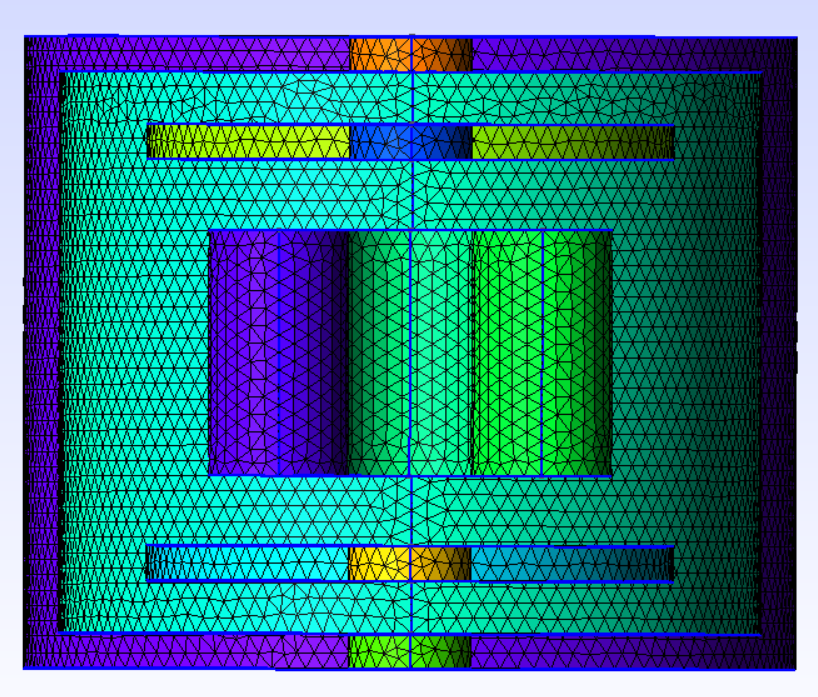
\includegraphics[width=\linewidth]{images/Coupe_quadrupole.png}
    \caption{Vue en coupe du maillage du quadrupole}
    \label{fig:coupe_quad}
\end{minipage}
\hspace{2cm}
\begin{minipage}{0.4\textwidth}
    \centering
    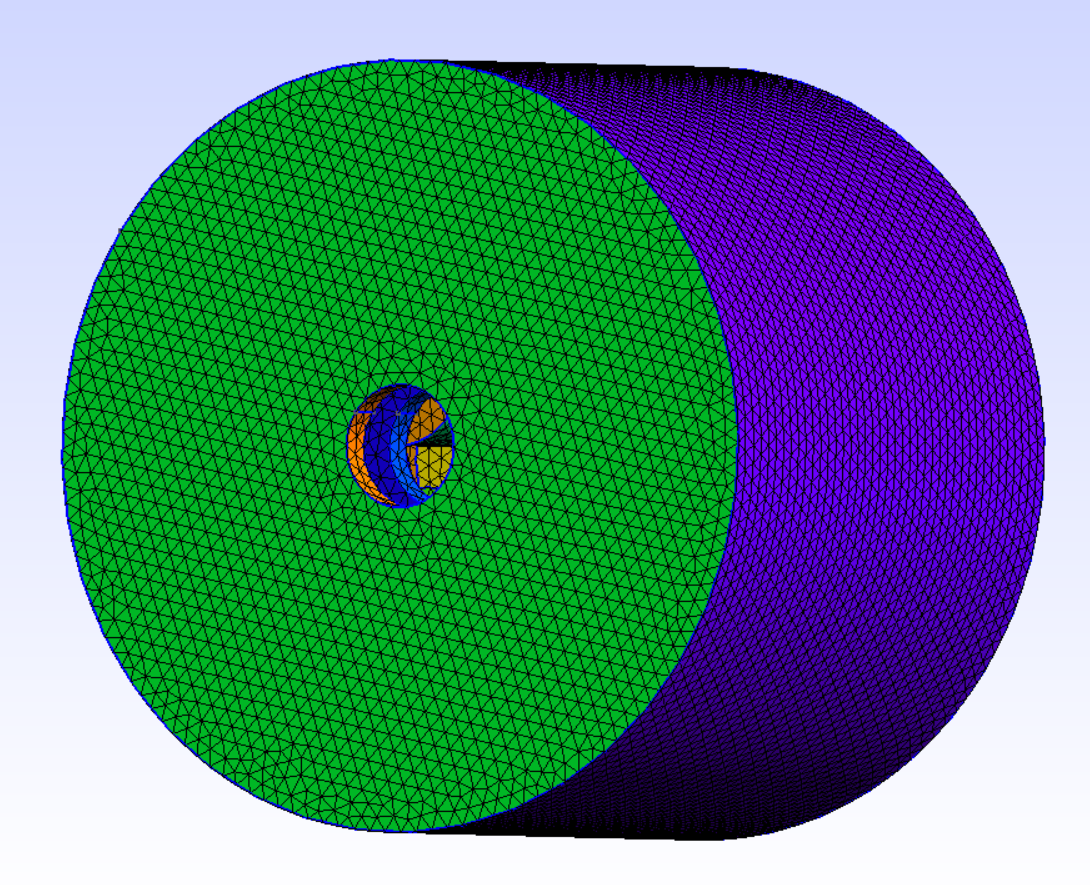
\includegraphics[width=\linewidth]{images/Quadrupole_shield.png}
    \caption{Vue du maillage du quadrupole}
    \label{fig:shield_quad}
\end{minipage}

\end{figure}

\subsection{Field calculation} 
Ce code permet d'importer le maillage et d'extraire le potentiel électrostatique en tout point du volume en utilisant la méthode des éléments de frontière (BEM).
L'application de cette méthode se fait à l'aide de la bibliothèque Python nommée BEMPP (Boundary Element Method Python Package).
\lstinputlisting[language=python]{../../Quadrupole_model/Field_calculation.py}

\subsection{Extraction data}
Ce code permet de récupérer toutes les variables créees dans le code Data.py et les données exportées lors de l'extraction du potentiel.
\lstinputlisting[language=python]{../../Quadrupole_model/Extraction_data.py}

\subsection{Multipolar decomposition}
Ce code permet de calculer les différentes composantes de la décomposition du potentiel.
\lstinputlisting[language=Python, extendedchars=false, inputencoding=utf8, literate=, basicstyle=\small\ttfamily, breaklines=true]{../../Quadrupole_model/Multipolar_decomposition.py}
Voici un graphique représentant les différentes composantes multipolaires le long de l'axe z: 
\begin{figure}[H]
\centering
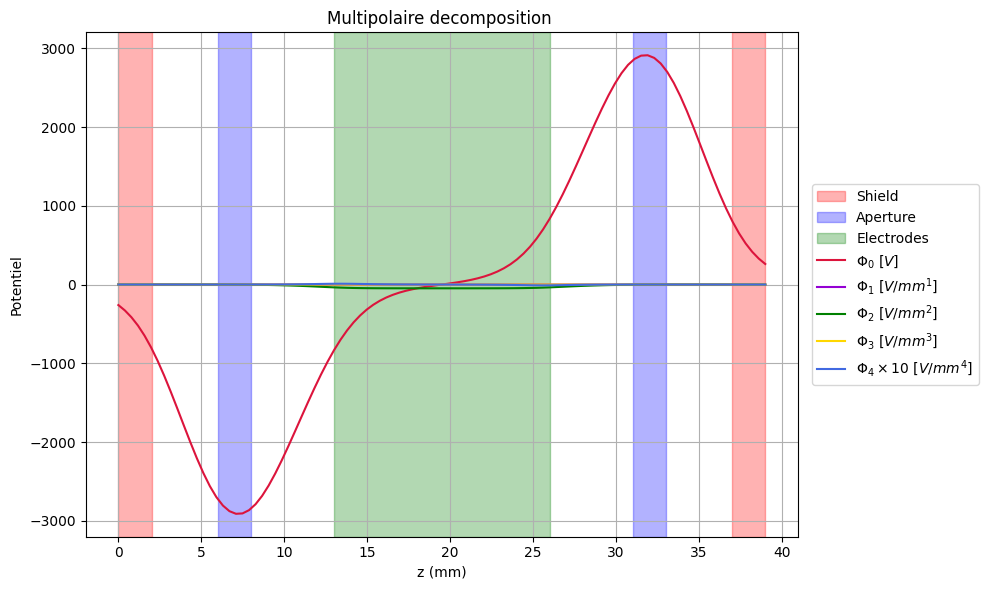
\includegraphics[width=1\linewidth]{images/décomposition_multipolaire.png} 
\caption{Graphique de la décomposition multipolaire}
\label{fig:decomposition}
\end{figure}



\subsection{Fit functions}
Ce code permet d'implémenter les fonctions de fit présentent dans le papier d'Okayama (Okayama et Kawakatsu, 1978) afin de vérifier si nos codes 
fonctionnent correctement.
\lstinputlisting[language=Python, extendedchars=false, inputencoding=utf8, literate=, basicstyle=\small\ttfamily, breaklines=true]{../../Quadrupole_model/Fit_functions.py}
Voici un graphique représentant les différentes composantes multipolaires normées ainsi que les fonctions de fit d'Okayam, le long de l'axe z: 
\begin{figure}[H]
\centering
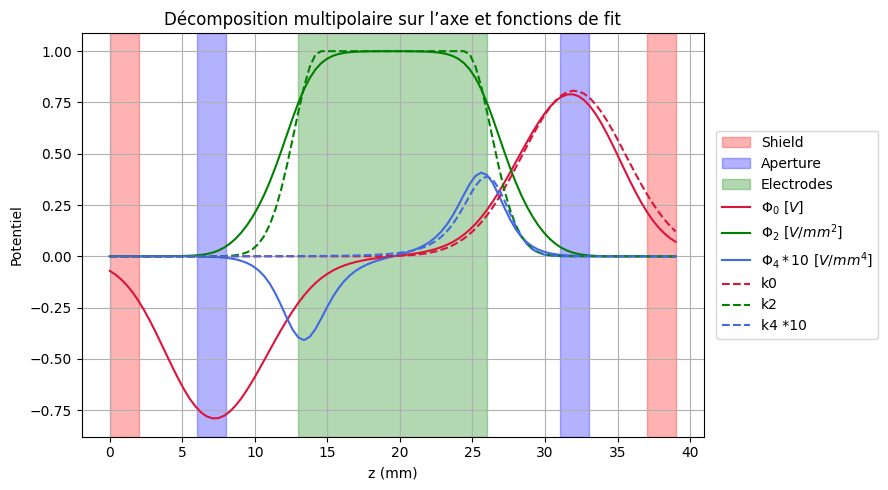
\includegraphics[width=1\linewidth]{images/fonction_fit.png} 
\caption{Graphique de la décomposition multipolaire et des fonctions de fit}
\label{fig:fitfunction}
\end{figure}



\subsection{Graphs}
Ce code permet d'afficher différents graphiques tels que la valeur des différentes composantes du potentiels le long de l'axe z.
\lstinputlisting[language=Python, extendedchars=false, inputencoding=utf8, literate=, basicstyle=\small\ttfamily, breaklines=true]{../../Quadrupole_model/Graphs.py}


\subsection{Paraxial}
Ce code permet de résoudre les équations de la trajectoire et donc d'obtenir le comportement des rayons d'électrons à travers le quadrupole.
\lstinputlisting[language=Python, extendedchars=false, inputencoding=utf8, literate=, basicstyle=\small\ttfamily, breaklines=true]{../../Quadrupole_model/paraxial.py}


\end{document}